\begin{frame}
	\frametitle{Terminologia}
	\begin{itemize}
	\item \textbf{Ipocentro}: luogo di origine del terremoto
	\item \textbf{Epicentro}: proiezione dell'ipocentro in superficie
	\item \textbf{Faglia}: frattura tra due placche
	\item \textbf{Sismografo}: dispositivo analogico per la misurazione delle onde sismiche, \textit{non più in uso}
	\item \textbf{Sismometro}: sistema di misurazione digitale/elettronico del terremoto
	\end{itemize}
\end{frame}
\begin{frame}
	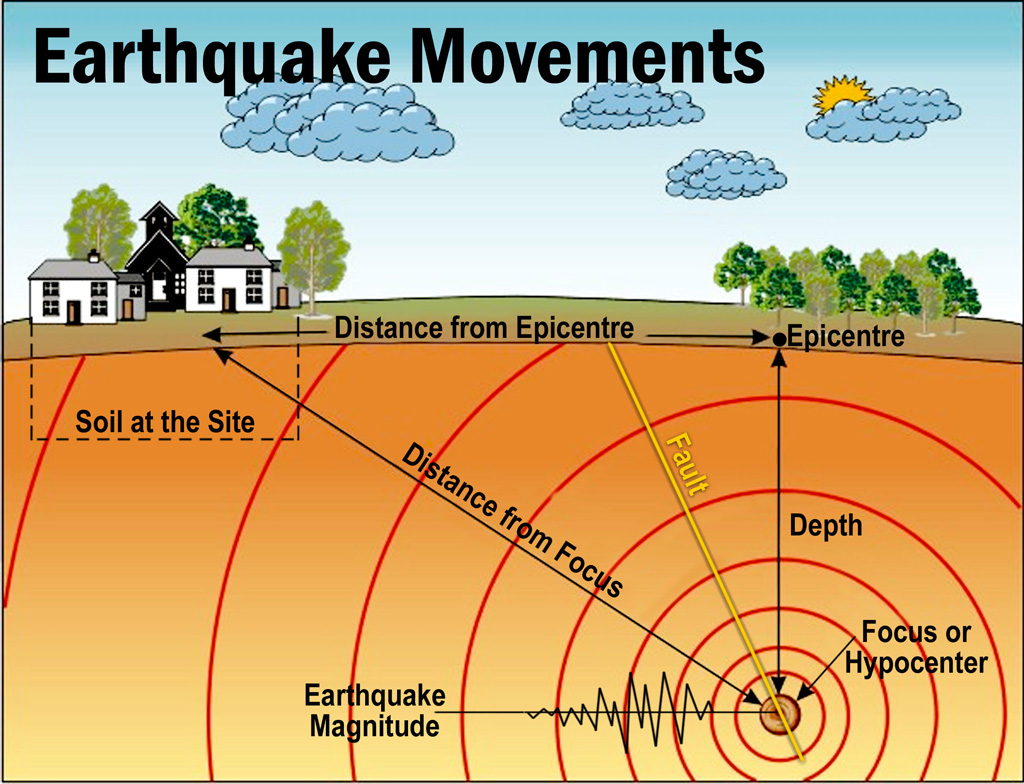
\includegraphics[keepaspectratio=true,width=0.8\paperwidth]{earthquake-points}
\end{frame}
